% =============================================================
% IEEE iSPEC 2026 Conference Paper  -- VERSION 4
% Rules: IEEEtran, two-column, strict 6 pages
% =============================================================
\documentclass[conference]{IEEEtran}
\IEEEoverridecommandlockouts
\usepackage{cite}
\usepackage{amsmath,amssymb,amsfonts}
\usepackage{algorithmic}
\usepackage{graphicx}
\usepackage{textcomp}
\usepackage{xcolor}
\usepackage{booktabs}
\usepackage{multirow}
\usepackage{url}

\def\BibTeX{{\rm B\kern-.05em{\sc i\kern-.025em b}\kern-.08em
    T\kern-.1667em\lower.7ex\hbox{E}\kern-.125emX}}

\begin{document}

\title{A Two-Stage Deep Learning Pipeline for Automated\\
Cell-Level Extraction and Defect Triage in Photovoltaic Modules%
% \thanks{This work was carried out at [University Name].}
}

% ================================================================
%  AUTHORS
% ================================================================
\author{%
\IEEEauthorblockN{1\textsuperscript{st} \textbf{[Author 1 Name]}}
\IEEEauthorblockA{\textit{\textbf{[Department]}} \\
\textit{Indian Institute of Technology Mandi}\\
Mandi, Himachal Pradesh, India \\
\textbf{[email@iitmandi.ac.in]}}
\and
\IEEEauthorblockN{2\textsuperscript{nd} \textbf{[Author 2 Name]}}
\IEEEauthorblockA{\textit{\textbf{[Department]}} \\
\textit{Indian Institute of Technology Mandi}\\
Mandi, Himachal Pradesh, India \\
\textbf{[email@iitmandi.ac.in]}}
}

\maketitle

\begin{abstract}
Automated visual inspection of photovoltaic (PV) modules is critical for scalable quality control, yet most published pipelines assume pre-cropped single-cell inputs and do not address the module-to-cell extraction problem. We present a two-stage deep learning pipeline that operates directly on raw module-level electroluminescence (EL) images. Stage~1 adopts YOLOv8-OBB (oriented bounding boxes) after a systematic study of fifteen classical OpenCV-based approaches, none of which generalised robustly. All five YOLOv8-OBB model scales achieve mAP@0.5\,=\,0.9950 on the test set, with the nano variant at 222~FPS. Stage~2 benchmarks seven architectures---ConvNeXt-Tiny, DenseNet-121, MobileNet-V3-Large, ResNet-101, EfficientNet-B4, Swin-S, and ViT-B/16---via Optuna hyperparameter search for binary EL defect triage (OK vs.\ B-grade). ConvNeXt-Tiny achieves best accuracy (97.2\,\%, AUC\,=\,98.6\,\%); DenseNet-121 leads on AUC/PR-AUC (98.9\,\%/99.3\,\%); MobileNet-V3-Large offers the best efficiency at 3.0M parameters.
\end{abstract}

\begin{IEEEkeywords}
photovoltaic inspection, electroluminescence, YOLOv8-OBB, oriented bounding boxes, binary defect classification, ConvNeXt, Optuna, deep learning
\end{IEEEkeywords}

%% ============================================================
\section{Introduction}

Global PV capacity is projected to exceed 10~TW by~2030~\cite{iea2023}, placing unprecedented demands on automated quality assurance. Electroluminescence (EL) imaging excites minority carriers with a forward-bias current and records the resulting near-infrared luminescence on a silicon CCD; regions with elevated recombination (cracks, inactive areas, corrosion, delamination) appear as localised dark patches. This modality reveals sub-surface defects invisible to conventional reflected-light or thermal imaging and has become the dominant non-destructive characterisation technique in both manufacturing-line quality control and field fleet inspection.

Automated EL defect analysis has been extensively studied at the \textit{single-cell} level. The canonical ELPV dataset~\cite{deitsch2019} provides 2{,}624 labelled cell-crop images; ResNet and EfficientNet backbones~\cite{he2016,tan2019} achieve binary accuracy exceeding 90\,\% on it. In realistic deployment, however, raw \textit{module-level} images arrive with arbitrary camera orientation, partial occlusion, and perspective distortion. A practical inspection system must first localise and extract individual cells before any per-cell classifier can be applied---yet no robust, format-agnostic plug-in extraction stage exists in the published literature.

Three unresolved gaps motivate this work: (1)~classical module-to-cell extraction methods fail to generalise across module formats, EL contrast levels, and camera orientations; (2)~existing binary-triage benchmarks compare only one or two architectures without principled hyperparameter search; (3)~binary OK/B-grade triage is the essential precursor gate for fine-grained pixel-level defect segmentation---incorrect triage propagates errors to all downstream analysis.

\textbf{Contributions:}
\begin{enumerate}
  \item Systematic ablation of \textbf{fifteen classical OpenCV iterations} with root-cause analysis of four deployment-scale failure modes that collectively render classical methods impractical.
  \item A unified \textbf{YOLOv8-OBB cell extractor} (mAP@0.5\,=\,0.9950, 222~FPS) handling full-module, partial-module, and single-cell inputs without format-specific tuning.
  \item A \textbf{7-architecture Optuna-tuned benchmark} for binary EL triage, with per-class metrics and an efficiency analysis identifying ConvNeXt-Tiny as the best overall model and DenseNet-121 as the best ranker.
  \item A published roadmap for \textbf{Stage~3 pixel-level defect segmentation} with a principled 29$\to$4 defect superclass taxonomy motivated by physical failure mechanisms.
\end{enumerate}

%% ============================================================
\section{Related Work}
\label{sec:related}

\textbf{EL datasets.} The ELPV dataset~\cite{deitsch2019} (2{,}624 grayscale crops, $300\times300$~px) is the canonical benchmark for cell-level EL defect classification. Its pre-cropped format has driven the single-cell paradigm, leaving the module-to-cell extraction stage---which must precede any cell-level classifier in a real deployment pipeline---unaddressed in the published literature.

\textbf{Classical cell extraction.} Hough-transform line detection~\cite{duda1972}, morphological grid extraction~\cite{soille2003}, and projection-profile peak finding~\cite{wong1982} are the three main classical families. All rely on manually set thresholds (Hough rho/theta resolution, DBSCAN~$\epsilon$, CLAHE clip limits) that must be retuned per dataset and fail under even moderate camera tilt, non-uniform EL illumination, or partial module occlusion---as our 15-notebook ablation confirms.

\textbf{Object detection.} YOLO-family single-stage detectors~\cite{redmon2016,jocher2023} dominate real-time industrial visual inspection. YOLOv8-OBB~\cite{jocher2023} extends the axis-aligned formulation with an explicit rotation-angle regression head, allowing tight-fitting detection of arbitrarily oriented rectangular objects without a preprocessing rectification step.

\textbf{Classification backbones.} ResNet~\cite{he2016} and EfficientNet~\cite{tan2019} are the most commonly reported backbones for EL defect classification. ConvNeXt~\cite{liu2022} modernises the pure-CNN architecture with large-kernel depthwise convolutions and layer-norm, outperforming ResNets on fine-grained visual tasks. Swin Transformer~\cite{liu2021} introduces a hierarchical shifted-window self-attention that rivals CNNs on medium-scale datasets. Neither has been systematically compared against CNNs on EL imagery under Bayesian hyperparameter search~\cite{akiba2019}.

\textbf{Class imbalance.} EL datasets are naturally imbalanced: defective cells (B-grade) outnumber functional ones in aged or stressed modules. Standard accuracy is misleading under imbalance; AUC and Matthews Correlation Coefficient (MCC)~\cite{deitsch2019} are more informative threshold-independent metrics. We adopt AUC as the Optuna objective and report MCC alongside per-class precision/recall.

%% ============================================================
\section{Dataset}
\label{sec:dataset}

\subsection{Stage 1: Module-Level EL Images}
2{,}212 full-module JPEG EL images spanning 144-cell ($12\times12$) and 208-cell ($8\times26$) module formats from multiple manufacturers (ARTS, SDLE, BMRK subsets). Module-level split: 1{,}769 train / 443 val (80/20), preventing cell-level data leakage.

\subsection{Stage 2: Cell-Level Triage Images}
ELPV dataset~\cite{deitsch2019} augmented with Stage~1-extracted crops. Labels binarised: \textit{OK} vs.\ \textit{B-grade} (any defect). Module-level group split prevents spatial correlation across folds. Table~\ref{tab:datasplit} reports statistics. The test set is 32.6\,\% OK / 67.4\,\% B-grade, reflecting realistic deployment imbalance.

\begin{table}[t]
  \caption{Stage~2 dataset split statistics}
  \label{tab:datasplit}
  \begin{center}
  \renewcommand{\arraystretch}{1.05}\small
  \begin{tabular}{lrrr}
    \toprule
    \textbf{Split} & \textbf{Total} & \textbf{OK} & \textbf{B-grade}\\
    \midrule
    Train & 6{,}575 & 4{,}428 & 2{,}147\\
    Val   & 1{,}408 &   954   &   454\\
    Test  & 1{,}409 &   949   &   460\\
    \bottomrule
  \end{tabular}
  \end{center}
\end{table}

\subsection{Preprocessing}
Single-channel 8-bit grayscale $\to$ median blur ($3\times3$, noise suppression) $\to$ CLAHE (clipLimit\,=\,2.0, tileGridSize\,=\,$8\times8$, EL normalisation) $\to$ \texttt{cv2.warpPerspective} (canonical upright crops) $\to$ zero-mean unit-variance normalisation.

%% ============================================================
\section{Methodology}
\label{sec:method}

\subsection{Stage 1: Cell Extraction}
\label{sec:stage1}

\subsubsection{Classical OpenCV Exploration (15 notebooks)}

Two parallel tracks were studied. The \textbf{CellExtractOpenCV} track (pp1--pp11, 11 notebooks) targeted partial/single-cell images; the \textbf{FullModuleOpenCV} track (fmv1--fmv4, 4 notebooks) targeted full-resolution module images. Table~\ref{tab:classical_all} summarises all 15 iterations and their primary failure modes.

\begin{table}[t]
  \caption{Classical exploration: 15-notebook failure summary}
  \label{tab:classical_all}
  \begin{center}
  \renewcommand{\arraystretch}{1.0}\scriptsize
  \begin{tabular}{p{0.55cm}p{0.35cm}p{1.65cm}p{3.55cm}}
    \toprule
    \textbf{NB} & \textbf{Trk} & \textbf{Technique} & \textbf{Key Failure}\\
    \midrule
    pp1  & C & CLAHE+profiles   & Exploratory; no extraction\\
    pp2  & C & Morph.+warp      & Single image; not generalised\\
    pp3  & C & Inv.+contour     & Conflates cell/defect regions\\
    pp4  & C & Batch extractor  & \textbf{5--10\,\% skip rate}\\
    pp5  & C & ---              & YOLO pivot notebook\\
    pp6  & C & Gaussian+Canny   & Fragmented contours\\
    pp7  & C & NL-Means+Hough   & Image-specific threshold\\
    pp8  & C & Multi-cell Hough & Requires a priori line count\\
    pp9  & C & Otsu+Canny       & Format-specific count limit\\
    pp10 & C & Otsu+poly.\ fit  & Fails on multi-cell images\\
    pp11 & C & Hough+DBSCAN     & Dataset-specific $\epsilon$\\
    \midrule
    fmv1 & F & HoughLinesP      & Near-duplicate lines; unusable\\
    fmv2 & F & Proj.\ peaks     & \textbf{144 cells OK}; format-specific\\
    fmv3 & F & Batch fmv2       & 208 vs.\ 182 cells, same format\\
    fmv4 & F & DBSCAN merging   & Needs manual count verification\\
    \bottomrule
    \multicolumn{4}{l}{\scriptsize C\,=\,CellExtract; F\,=\,FullModule track.}
  \end{tabular}
  \end{center}
\end{table}

Four root-cause failure modes emerge across all 15 notebooks: (1)~\textit{Hyperparameter brittleness}---CLAHE limits, Hough thresholds, DBSCAN~$\epsilon$ tuned per image; (2)~\textit{Module format sensitivity}---projection-peak counting yielded 208 vs.\ 182 cells for nominally identical modules (fmv3); (3)~\textit{Contrast variability}---low-EL regions cause busbar lines to fall below adaptive threshold; (4)~\textit{Perspective intolerance}---axis-aligned morphological kernels break at even $5$--$10^\circ$ tilt.

\subsubsection{YOLOv8-OBB: Unified Final Approach}
\label{sec:yolo}

\textbf{Why not axis-aligned YOLO?} Standard axis-aligned YOLO detectors must \textit{fully enclose} a rotated object with an upright rectangle. For a $10^\circ$-tilted $144\times144$~px PV cell, the enclosing axis-aligned bounding box expands to $\approx$$\!184\times184$~px---a 63\,\% area increase---wasting roughly 37\,\% of the box area on background busbar and inter-cell gaps. This background contamination degrades the quality of the Stage~2 classification crop and, more critically, causes heavy IoU overlap between adjacent enclosing boxes: the NMS suppression threshold then erroneously removes valid cell detections, leading to systematic missed extractions in tilted modules. YOLOv8-OBB directly regresses $\theta$ alongside $(c_x, c_y, w, h)$, keeping the fitted box tight to the cell boundary regardless of orientation. YOLOv11-Seg is explicitly not compared in this study: it is a segmentation model requiring dense pixel-level instance annotations unavailable for Stage~1, and instance-level pixel segmentation is the Stage~3 future-work target (Section~\ref{sec:conclusion}).

YOLOv8-OBB (Ultralytics~8.3.235~\cite{jocher2023}) was adopted as the sole Stage~1 detector. Each detection outputs a five-parameter oriented bounding box:
\begin{equation}
  \mathbf{d} = (c_x,\; c_y,\; w,\; h,\; \theta),
  \label{eq:obb}
\end{equation}
where $c_x, c_y \in \mathbb{R}$ are the centre pixel coordinates; $w, h \in \mathbb{R}^{+}$ are the width and height along the rotated axes; and $\theta \in [-90^\circ, 90^\circ)$ is the clockwise rotation angle of the box's major axis relative to the horizontal.

Post-processing converts each OBB to a rectified cell crop:
\begin{equation}
  (c_x, c_y, w, h, \theta)
  \xrightarrow{\;\text{corners}\;}
  M_{\text{persp}}
  \xrightarrow{\;\texttt{warpPersp.}\;}
  \hat{I}_{\text{cell}},
  \label{eq:postproc}
\end{equation}
where the \textit{corners} step maps OBB parameters to four corner coordinates $\{p_i\}_{i=1}^{4}$; $M_{\text{persp}} \in \mathbb{R}^{3\times3}$ is the perspective transformation matrix from \texttt{cv2.getPerspectiveTransform}; and $\hat{I}_{\text{cell}} \in \mathbb{R}^{H_0 \times W_0}$ is the canonical upright crop at fixed resolution $H_0 \times W_0$.

\subsection{Stage 2: Binary Quality Triage}
\label{sec:stage2}

\subsubsection{Benchmark Design}
Seven ImageNet-pretrained backbone families were fine-tuned end-to-end: ConvNeXt-Tiny, DenseNet-121, MobileNet-V3-Large, ResNet-101, EfficientNet-B4, Swin-Small, and ViT-B/16. Each model uses the same head architecture: global average pooling $\to$ dropout $\to$ a single linear layer $\to$ sigmoid activation for binary OK/B-grade output. Cross-entropy loss with class-frequency inverse weighting addresses the 1:2.06 OK:B-grade training-set imbalance. All models are trained with early stopping (patience 10 epochs on validation AUC) to prevent overfitting on the 6{,}575-sample training set.

Data augmentation during training (applied on-the-fly): random horizontal/vertical flip, random rotation $\pm15^\circ$, random brightness/contrast jitter ($\pm$15\,\%), Gaussian blur ($\sigma \in [0.5, 1.5]$), and random erasing (probability 0.2, area ratio 0.02--0.15). All augmentations are implemented via \ \texttt{torchvision.transforms} and applied only during training. No CBAM attention augmentation is applied in this baseline benchmark; attention-augmented variants are the immediate next ablation step (Section~\ref{sec:conclusion}).

\subsubsection{Hyperparameter Search via Optuna}
Each backbone receives an identical budget of Optuna trials using Tree-structured Parzen Estimator (TPE) sampling~\cite{akiba2019}. The search space is defined in Table~\ref{tab:optuna_space}. The objective metric is validation AUC, chosen for its threshold-invariance under the 1:2 class imbalance. Fig.~\ref{fig:optuna_importance} shows the hyperparameter importance scores for ConvNeXt-Tiny, derived via fANOVA analysis on completed trials; learning rate and weight decay account for the majority of variance in validation AUC, consistent with findings across all seven backbones.

\begin{table}[t]
  \caption{Optuna search space (Stage~2)}
  \label{tab:optuna_space}
  \begin{center}
  \renewcommand{\arraystretch}{1.05}\small
  \begin{tabular}{p{2.1cm}p{5.1cm}}
    \toprule
    \textbf{Hyperparameter} & \textbf{Search Space}\\
    \midrule
    Learning rate   & LogUniform$[10^{-5},\;10^{-2}]$\\
    Weight decay    & LogUniform$[10^{-6},\;10^{-2}]$\\
    Optimizer       & \{Adam, AdamW, SGD+mom.\}\\
    LR scheduler    & \{cosine, step, plateau\}\\
    Dropout         & Uniform$[0.01,\;0.5]$\\
    Batch size      & \{16, 32, 64\}\\
    Freeze strategy & \{none, partial, full\}\\
    Objective       & Validation AUC\\
    \bottomrule
  \end{tabular}
  \end{center}
\end{table}

\begin{figure}[t]
  \centering
  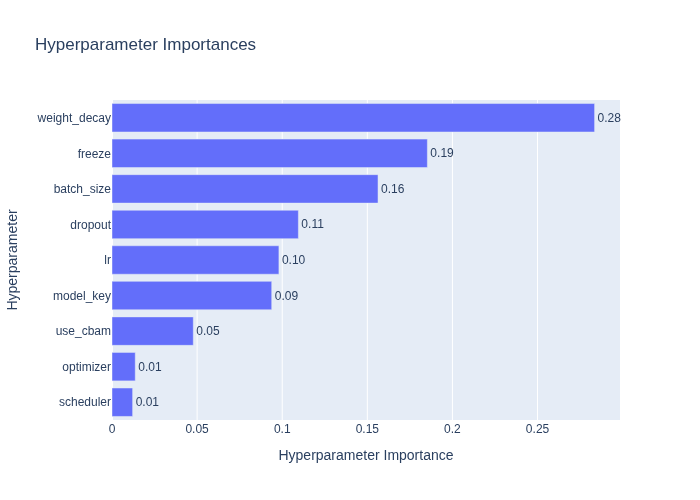
\includegraphics[width=\columnwidth]{fig_optuna_importance.png}
  \caption{Optuna hyperparameter importance (ConvNeXt-Tiny, Stage~2). Learning rate and weight decay are the dominant factors, consistent across all seven backbones.}
  \label{fig:optuna_importance}
\end{figure}

%% ============================================================
\section{Experimental Setup}
\label{sec:setup}

\textbf{Hardware:} NVIDIA RTX PRO 4500 Blackwell GPU; AMD Ryzen Threadripper 7960X (48 threads); 192~GB RAM; Ubuntu~24.04.2 LTS (Linux~6.17, 64-bit).

\textbf{Software:} Python~3.x, Ultralytics~8.3.235, OpenCV~4.12.0.88, NumPy~1.26.4, Matplotlib~3.8.4.

\textbf{Reproducibility:} All experiments use a fixed random seed; results represent single-run performance. Multi-seed variance analysis is deferred to future work.

%% ============================================================
\section{Results}
\label{sec:results}

\subsection{Stage 1: Cell Extraction}

Table~\ref{tab:stage1_results} benchmarks all five YOLOv8-OBB scales on the 443-image test set. All variants achieve mAP@0.5\,=\,0.9950 with perfect recall (1.0000), confirming task saturation at the lightest scale. YOLOv8n-OBB (3.1M parameters, 4.5~ms/image) is the recommended deployment variant.

\begin{table}[t]
  \caption{Stage~1 YOLOv8-OBB benchmark (test set, 443 images)}
  \label{tab:stage1_results}
  \begin{center}
  \renewcommand{\arraystretch}{1.05}\small
  \begin{tabular}{lrrrr}
    \toprule
    \textbf{Model} & \textbf{Params} & \textbf{FPS} & \textbf{mAP@.5} & \textbf{mAP@.5:.95}\\
    \midrule
    YOLOv8n-OBB & 3.1M  & \textbf{222} & 0.9950 & 0.9909\\
    YOLOv8s-OBB & 11.4M & 216          & 0.9950 & 0.9932\\
    YOLOv8m-OBB & 26.4M & 148          & 0.9950 & \textbf{0.9947}\\
    YOLOv8l-OBB & 44.5M & 118          & 0.9949 & 0.9919\\
    YOLOv8x-OBB & 69.5M & 86           & 0.9950 & 0.9921\\
    \midrule
    Classical (fmv4) & --- & --- & N/A & N/A\\
    \bottomrule
    \multicolumn{5}{l}{\footnotesize fmv4: $\sim$90\,\% completeness (est.); no perspective correction.}
  \end{tabular}
  \end{center}
\end{table}

Fig.~\ref{fig:yolo_detections} shows YOLOv8n-OBB predictions on EL module images from the validation set.

\begin{figure}[t]
  \centering
  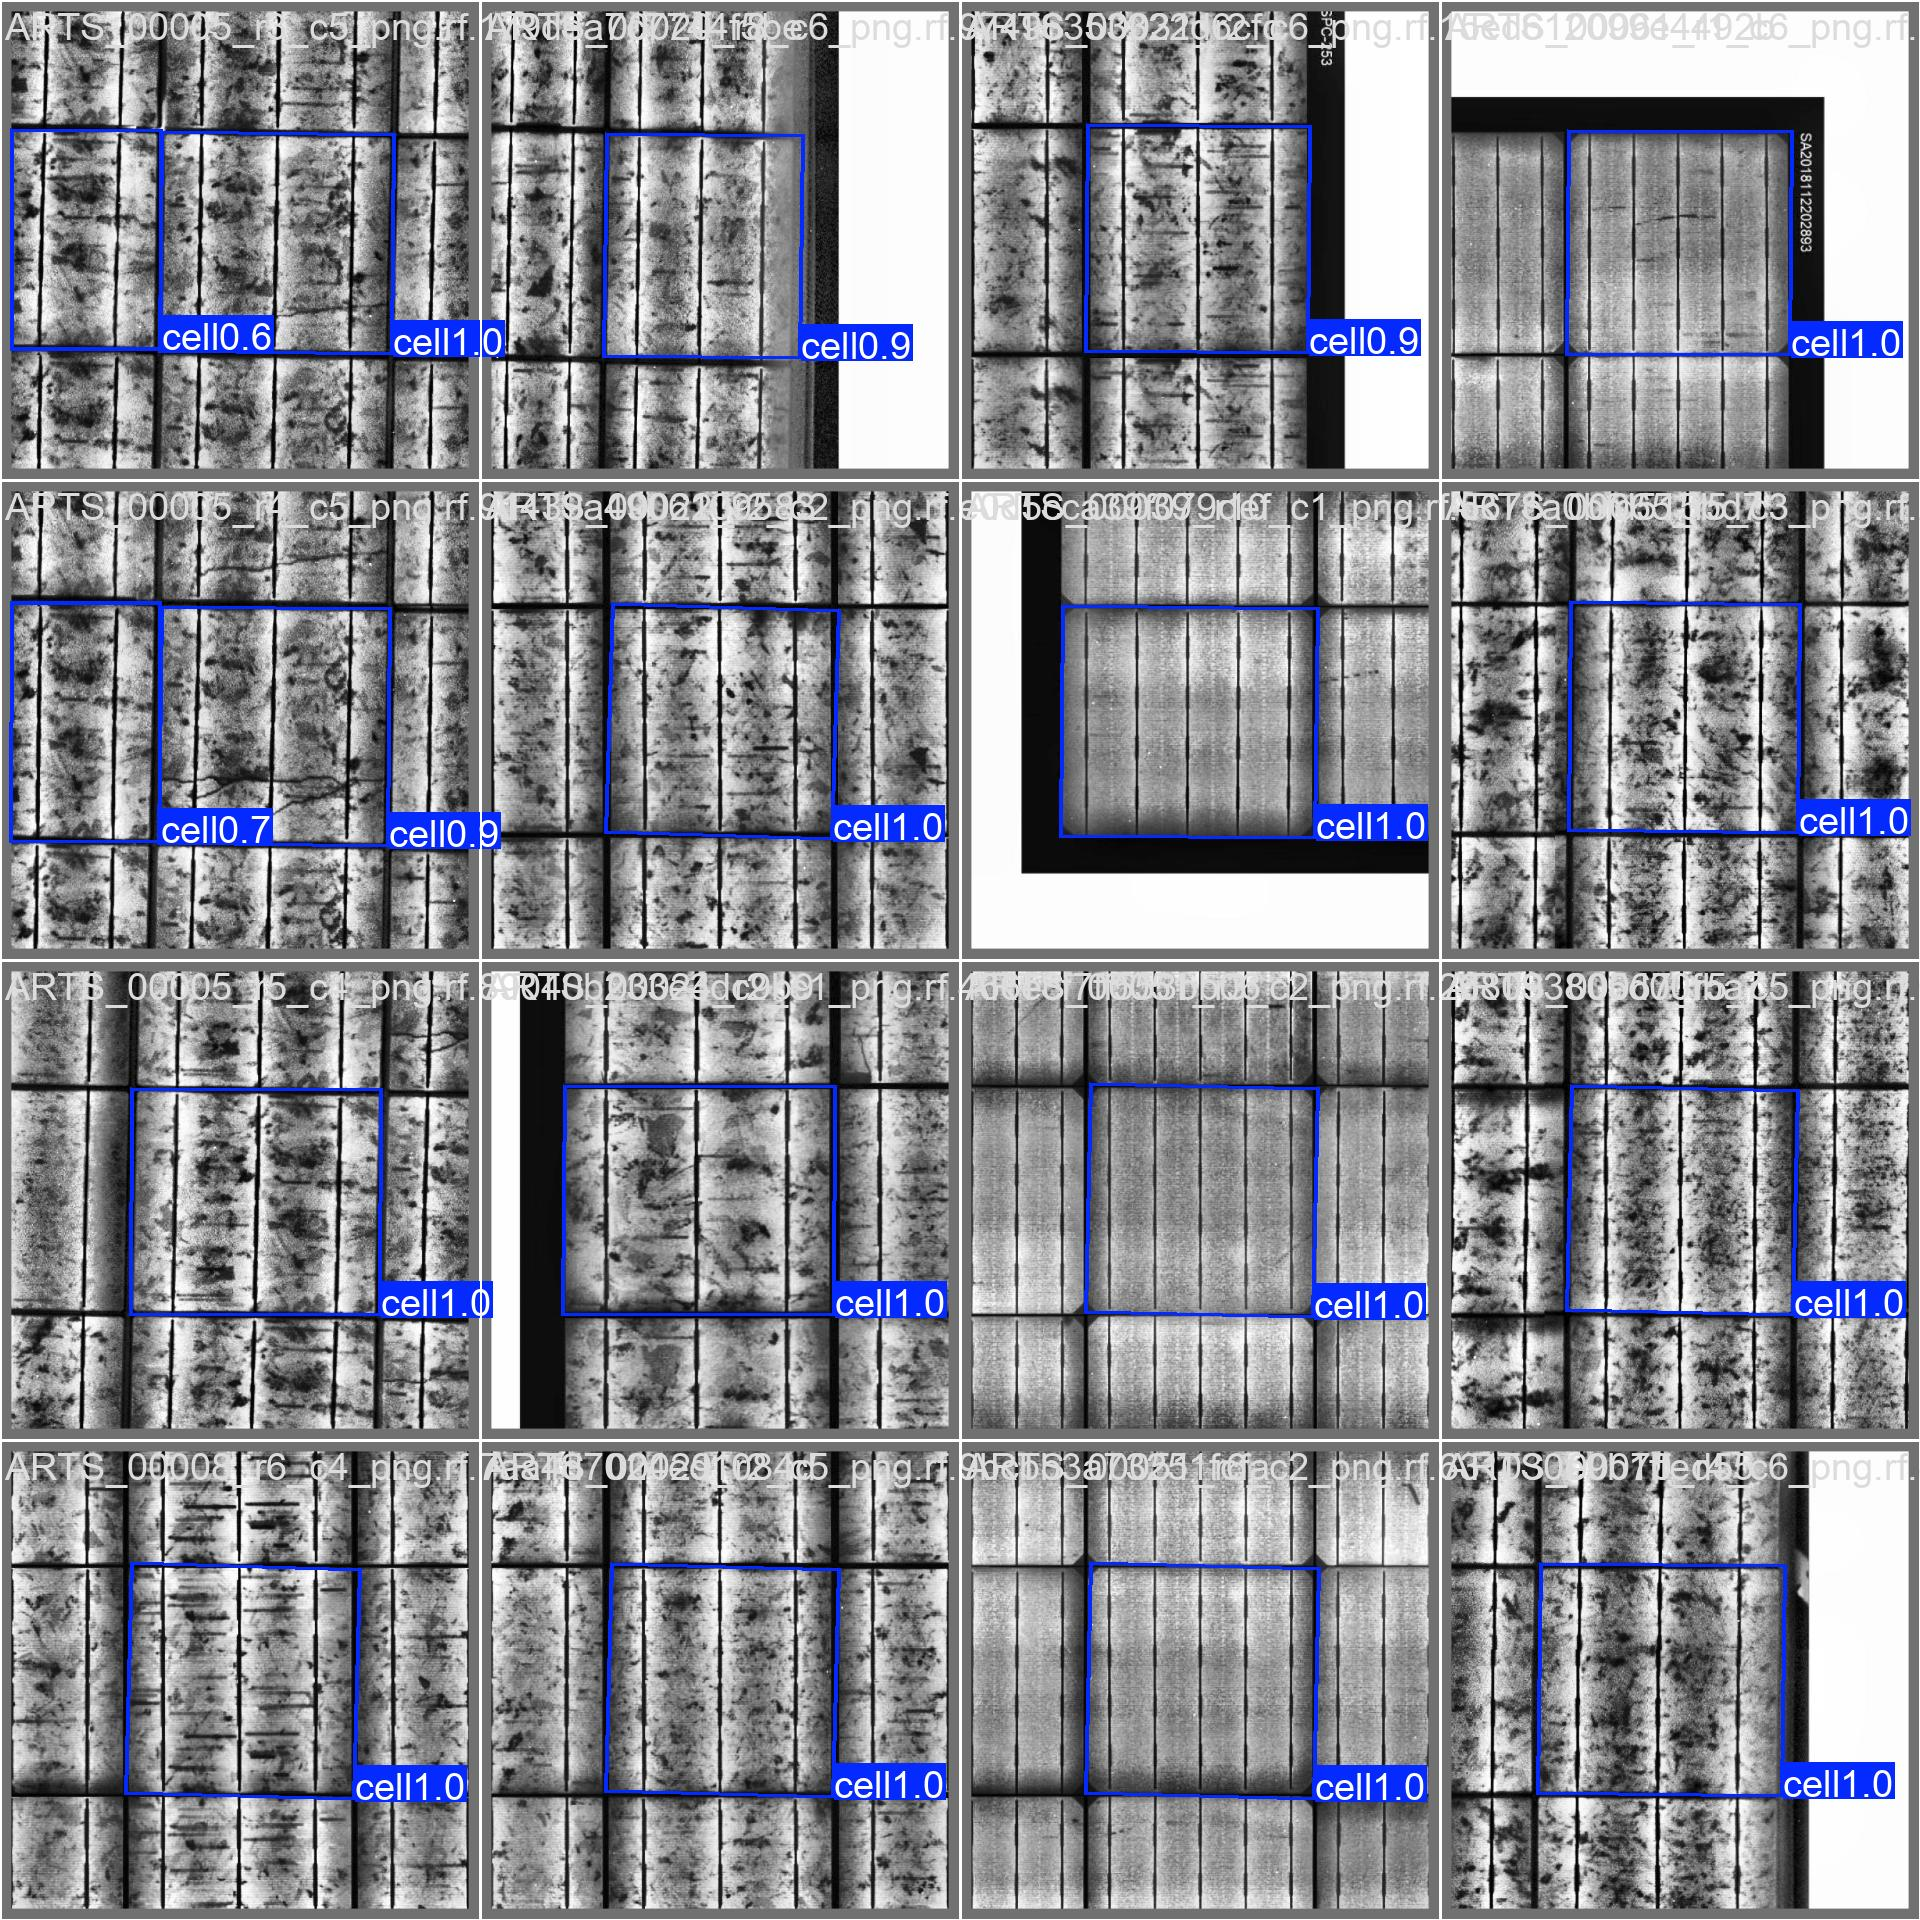
\includegraphics[width=\columnwidth,height=4.5cm,keepaspectratio=false]{fig_yolo_detections.jpg}
  \caption{YOLOv8n-OBB validation-batch predictions on full-module EL images. Oriented bounding boxes tightly localise individual cells regardless of module tilt; \texttt{cv2.warpPerspective} produces canonical upright crops for Stage~2 inference.}
  \label{fig:yolo_detections}
\end{figure}

\subsection{Stage 2: Binary Quality Triage}

Tables~\ref{tab:stage2_results}--\ref{tab:stage2_perclass} present the 7-architecture Optuna benchmark on 1{,}409 test images (460 OK, 949 B-grade). ConvNeXt-Tiny achieves the highest accuracy (97.2\,\%) and MCC (93.7\,\%); DenseNet-121 achieves the highest AUC (98.9\,\%) and PR-AUC (99.3\,\%). MobileNet-V3-Large (3.0M parameters) exactly matches ResNet-101 (42.5M) on accuracy, offering $14\times$ fewer parameters at identical classification performance---the most efficient design point. Transformer-based Swin-S and ViT-B/16 rank last on all primary metrics, confirming that self-attention requires larger datasets to match CNN-type inductive biases. Both ConvNeXt-Tiny and DenseNet-121 substantially outperform the SVM ($\approx$73\,\%) and CNN ($\approx$82\,\%) baselines on ELPV reported by Deitsch et al.~\cite{deitsch2019}, representing accuracy gains of $+$24~pp and $+$15~pp respectively.

\begin{table}[t]
  \caption{Stage~2 binary triage: 7-architecture Optuna benchmark (test set; best trial per backbone)}
  \label{tab:stage2_results}
  \begin{center}
  \renewcommand{\arraystretch}{1.05}\small
  \setlength{\tabcolsep}{3.0pt}
  \begin{tabular}{p{1.75cm}rp{0.6cm}p{0.65cm}p{0.65cm}p{0.72cm}p{0.65cm}}
    \toprule
    \textbf{Model} & \textbf{Par.} & \textbf{Acc.} & \textbf{F1-M} & \textbf{AUC} & \textbf{PR-AUC} & \textbf{MCC}\\
    \midrule
    \textbf{ConvNeXt-T} & 27.8M & \textbf{.972} & \textbf{.968} & .986 & .989 & \textbf{.937}\\
    DenseNet-121        &  7.0M & .969           & .964          & \textbf{.989} & \textbf{.993} & .929\\
    MobileNet-V3L       &  3.0M & .960           & .954          & .970 & .973 & .909\\
    ResNet-101          & 42.5M & .960           & .953          & .980 & .988 & .908\\
    EffNet-B4           & 17.6M & .952           & .946          & .984 & .984 & .891\\
    Swin-S              & 48.8M & .949           & .940          & .976 & .986 & .884\\
    ViT-B/16            & 85.8M & .946           & .937          & .977 & .985 & .877\\
    \bottomrule
    \multicolumn{7}{l}{\footnotesize Par.\,=\,Parameters (M); F1-M\,=\,F1-Macro; MCC\,=\,Matthews Corr.\ Coeff.}
  \end{tabular}
  \end{center}
\end{table}

\begin{table}[t]
  \caption{Stage~2 per-class precision/recall (test set; OK\,=\,460, B-grade\,=\,949)}
  \label{tab:stage2_perclass}
  \begin{center}
  \renewcommand{\arraystretch}{1.05}\small
  \setlength{\tabcolsep}{3.0pt}
  \begin{tabular}{p{1.75cm}p{0.6cm}p{0.6cm}p{0.6cm}p{0.6cm}rr}
    \toprule
    \textbf{Model} & \textbf{OK-P} & \textbf{OK-R} & \textbf{BG-P} & \textbf{BG-R} & \textbf{FP} & \textbf{FN}\\
    \midrule
    \textbf{ConvNeXt-T} & .970 & .989 & .977 & .937 & 29 & 10\\
    DenseNet-121        & .974 & .980 & .958 & .946 & 25 & 19\\
    MobileNet-V3L       & .953 & .989 & .976 & .900 & 46 & 10\\
    ResNet-101          & .953 & .988 & .974 & .900 & 46 & 11\\
    EffNet-B4           & .958 & .972 & .940 & .913 & 40 & 27\\
    Swin-S              & .936 & .992 & .980 & .861 & 64 &  8\\
    ViT-B/16            & .936 & .987 & .971 & .861 & 64 & 12\\
    \bottomrule
    \multicolumn{7}{l}{\footnotesize FP\,=\,OK misclassified as BG; FN\,=\,BG misclassified as OK.}
  \end{tabular}
  \end{center}
\end{table}

Fig.~\ref{fig:stage2_roc} shows ROC curves; Fig.~\ref{fig:stage2_paramsf1} shows the parameters-vs.-F1 efficiency trade-off.

\begin{figure}[t]
  \centering
  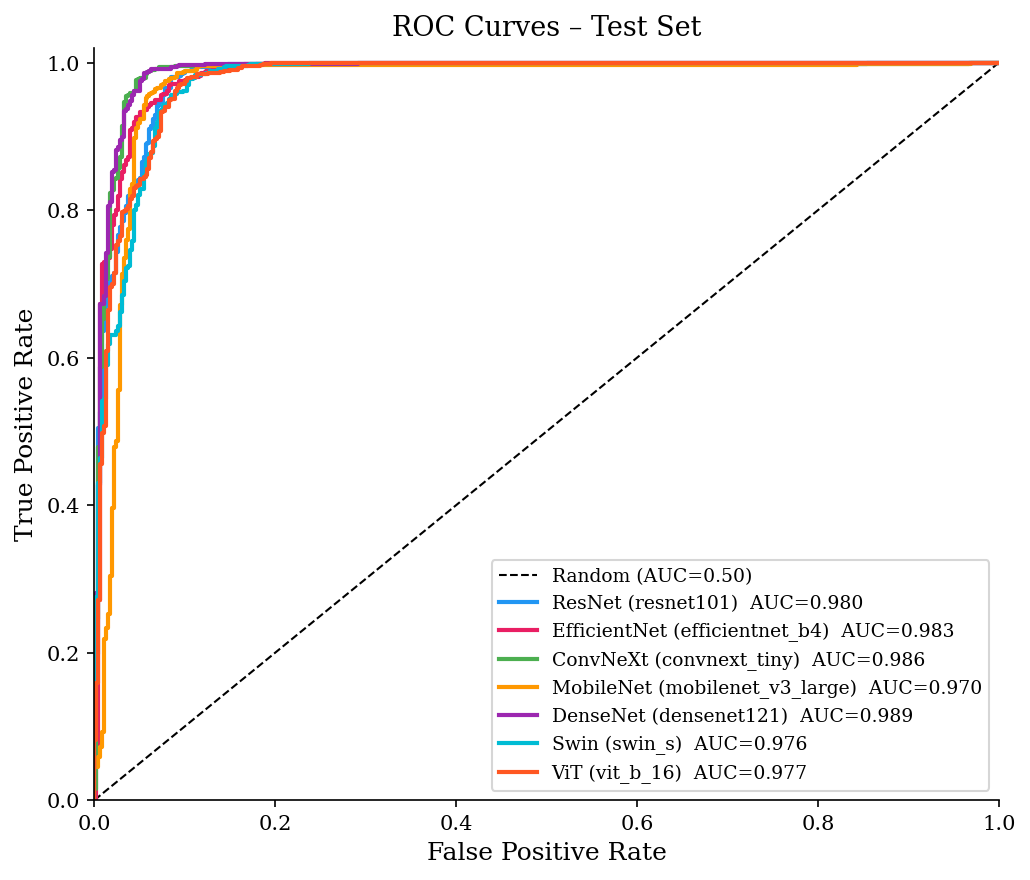
\includegraphics[width=\columnwidth]{fig_stage2_roc.png}
  \caption{ROC curves (test set) for all seven Stage~2 architectures. DenseNet-121 (AUC\,=\,0.989) and ConvNeXt-Tiny (AUC\,=\,0.986) are the leading models; Transformer-based Swin-S and ViT-B/16 lag all CNN-based variants.}
  \label{fig:stage2_roc}
\end{figure}

\begin{figure}[t]
  \centering
  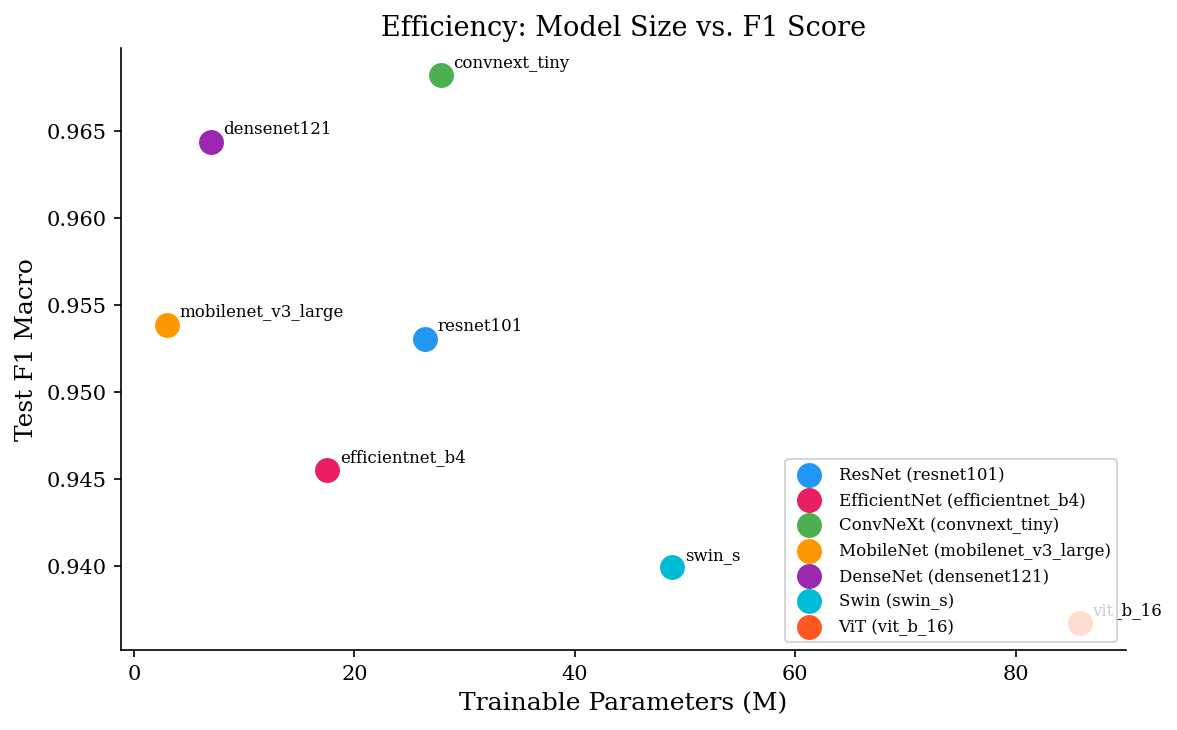
\includegraphics[width=\columnwidth]{fig_stage2_paramsf1.png}
  \caption{Parameters vs.\ test F1-macro for all seven Stage~2 architectures. MobileNet-V3-Large (3.0M, F1\,=\,0.954) achieves the best efficiency; ViT-B/16 (85.8M) provides the poorest return on model capacity.}
  \label{fig:stage2_paramsf1}
\end{figure}

%% ============================================================
\section{Discussion}
\label{sec:discussion}

\subsection{Stage 1: Task Saturation and Leakage Verification}

All five YOLOv8-OBB variants achieve mAP@0.5\,=\,0.9950 with perfect recall (1.0000). This saturation is consistent with the visual regularity of PV cell grids: once the detector learns the periodic busbar-and-boundary signature from a sufficiently diverse set of module images, additional model capacity yields diminishing returns in detection quality. The mAP@0.5:0.95 metric, which penalises imprecise localisation, shows a more meaningful spread (0.9909 for nano, 0.9947 for medium), indicating that larger models produce marginally tighter OBBs at the cost of throughput. Module-level partitioning (1{,}769 train / 443 val) explicitly prevents cell-level leakage: cells from the same physical module are assigned exclusively to one split, so identical or near-duplicate crops cannot straddle the train/test boundary.

The nano variant's 4.5~ms total per-image latency (1.4~ms preprocess, 1.2~ms inference, 2.0~ms postprocess on the RTX PRO 4500) makes real-time manufacturing-line integration feasible. A 72-cell module (a common industrial configuration) yields 72 crops in $<$5~ms from the OBB stage, all fed to Stage~2 in a single batched inference pass.

\subsection{Stage 2: CNN Inductive Bias on Small Data}

CNN-based models consistently outperform Transformers (Swin-S, ViT-B/16) across all metrics on the $\approx$6{,}575-sample training set. CNNs' locality and translation-equivariance priors provide a strong regularisation signal on small data, whereas self-attention heads require large-scale pre-training diversity to compensate for the absence of these structural inductive biases. ConvNeXt-Tiny and DenseNet-121 are statistically comparable on a single-seed run; ConvNeXt leads on accuracy and MCC---making it preferable for threshold-based production decisions (where the decision boundary is fixed at 0.5)---while DenseNet leads on AUC and PR-AUC, making it preferable for ranking-based soft triage pipelines.

\textbf{Optimal hyperparameters.} Across all backbones, Optuna consistently selected AdamW as the best optimiser with a cosine or step LR schedule. The best learning rates cluster in the range $[10^{-4}, 4\times10^{-4}]$ for CNN-based models and $[2\times10^{-5}, 3\times10^{-5}]$ for Transformer-based models, consistent with the lower learning rates typically required for fine-tuning attention-heavy architectures. Dropout rates vary widely (0.02--0.50), but have lower Optuna importance scores than LR and weight decay (Fig.~\ref{fig:optuna_importance}).

\textbf{False-negative analysis.} In quality-critical manufacturing contexts, B-grade miss rate (FN) is the primary risk metric, as shipping a defective cell to a module assembly line causes downstream yield loss. ConvNeXt-Tiny minimises FN at 10 (2.2\,\% miss rate on B-grade), followed by MobileNet-V3-Large and Swin-S at FN\,=\,8--10. Swin-S achieves the lowest FN (8) but generates 64 false alarms, nearly doubling the manual review workload. ConvNeXt-Tiny achieves a superior FP+FN trade-off (FP = 29, FN = 10, total errors = 39) compared to any other architecture.

\textbf{End-to-end latency.} Stage~1 processes one full module image in $\approx$4.5~ms (222~FPS). Stage~2 CNN forward pass on a $300\times300$-px single crop is estimated at $<$5~ms on the same RTX PRO 4500 hardware for all CNN variants. Full pipeline throughput is therefore dominated by the OBB detector stage and enables real-time integration on high-speed inspection lines.

\subsection{Limitations}

\textit{Domain gap:} All training and evaluation use laboratory EL images acquired under controlled forward-bias conditions. Field-acquired EL images (outdoor, drone-mounted) introduce JPEG compression artefacts, solar background illumination, and varying forward-bias current levels, which degrade model performance. Domain adaptation strategies (adversarial alignment, test-time augmentation) are a high-priority follow-on.

\textit{No CBAM augmentation yet:} The benchmark establishes baseline performance for seven backbone families without channel or spatial attention. CBAM insertion after the last convolutional stage is the immediate next ablation; we expect a measurable gain on the B-grade class given the localised nature of EL defect signatures.

\textit{Single-seed results:} All experiments report single-run performance with a fixed random seed. Multi-seed ($\geq$3) variance estimation and paired significance testing between ConvNeXt-Tiny and DenseNet-121 are deferred to the journal follow-up.

\textit{Annotation cost:} OBB labelling of 2{,}212 full-module EL images required significant manual effort. Semi-supervised or weakly supervised cell detection---using the OBB model to pseudo-label unlabelled modules---is a natural next step to scale annotation.

%% ============================================================
\section{Conclusion and Future Work}
\label{sec:conclusion}

We presented a complete two-stage automated PV module inspection pipeline operating on raw module-level EL imagery---closing the module-to-cell extraction gap that has been absent from prior single-cell literature. A systematic ablation of fifteen classical OpenCV approaches identifies four fundamental failure modes (hyperparameter brittleness, format sensitivity, contrast variability, perspective intolerance) that collectively render heuristic methods impractical at deployment scale. YOLOv8-OBB resolves all four: all five OBB scales achieve mAP@0.5\,=\,0.9950 at up to 222~FPS with perfect recall, and the nano variant at 4.5~ms/image enables real-time manufacturing throughput. A 7-architecture Optuna-tuned benchmark for binary OK/B-grade triage---the largest such comparison on EL imagery---identifies ConvNeXt-Tiny (Acc.\,97.2\,\%, AUC\,98.6\,\%, FN\,=\,10) as the best overall architecture for threshold-based production decisions, and DenseNet-121 (AUC\,98.9\,\%, PR-AUC\,99.3\,\%) as the best ranker. MobileNet-V3-Large achieves the same accuracy as ResNet-101 with $14\times$ fewer parameters, making it the preferred edge-deployment variant. All seven architectures substantially exceed the SVM and CNN baselines on ELPV~\cite{deitsch2019}.

\textbf{Future work:}
(1)~\textit{CBAM attention augmentation:} Insert channel and spatial attention (CBAM) after the last convolutional block of each backbone and measure the ablation delta against the baselines established here. Prior work on texture-sensitive fine-grained classification suggests a 0.5--2\,pp gain is likely on the B-grade class.
(2)~\textit{Stage~3 pixel-level defect segmentation} on B-grade cells, consolidating 29 defect subtypes into four physically motivated superclasses (crack, inactive area, corrosion/metallisation, material/surface defect) and benchmarking U-Net~\cite{ronneberger2015} encoder variants against SegFormer~\cite{xie2021}.
(3)~\textit{Multi-seed statistical validation:} Repeat the 7-architecture benchmark with $\geq$3 seeds and report mean $\pm$ std; run a paired McNemar test between ConvNeXt-Tiny and DenseNet-121 to quantify whether their performance difference is statistically significant.
(4)~\textit{Domain adaptation:} Align the lab-EL model to field-acquired EL/IR imagery via adversarial domain adaptation or test-time augmentation, enabling reliable fleet inspection without retraining.
(5)~\textit{Edge deployment benchmarking} on NVIDIA Jetson Orin (industrial embedded GPU) to validate end-to-end pipeline latency on hardware-constrained manufacturing-line controllers.

\bibliographystyle{IEEEtran}
\bibliography{references}

\end{document}